\label{principal_neccessity}

Покажем на модельном примере необходимость руководителя команды 
\cite{holmstrom1982moral}.

Пусть результат работы в команды задается производственной функцией $Q=Q(a_1,\dots,a_n)$ 
c положительными первыми производными $\frac{\partial Q}{\partial x_i} >0$ и матрицей второй производных с условиями:
\begin{equation}
    \frac{\partial^2 Q}{\partial a^2_i} <0, \quad \frac{\partial^2 Q}{\partial a_i a_j} > 0,
\end{equation}
задающие рост совместного вклада игроков $a$ с возрастанием участия агентов.

Оплата труда игроков $\mathbf{w}=(w_1, \dots, w_n)$ выполняется согласно контракту на основании
произведенной продукции $\mathbf{w} = \mathbf{w}(Q)$. В базовой постановке отсутствие принципала
распределение дохода между агентами считается эффективным:
\begin{equation}
    \sum_{i=1}^n \omega_i(Q) =Q 
\end{equation}

Агенты считаются рациональными и принимают решения c целью
максимизации функции утилитарности, заданной разностью дохода $\omega_i$ и вклада усилий $a_i$:
\begin{equation}
    u_i = $\omega_i$ - g_i(a_i),
\end{equation}
где функция тяжести труда (\texit{англ.} disutility) $g_i$ считается выпуклой и строго монотонной. $\frac{d g_i}{d a} >0 , \frac{d^2 g_i}{d^2 a} >= 0$.
\begin{figure}[h]
    \centering
    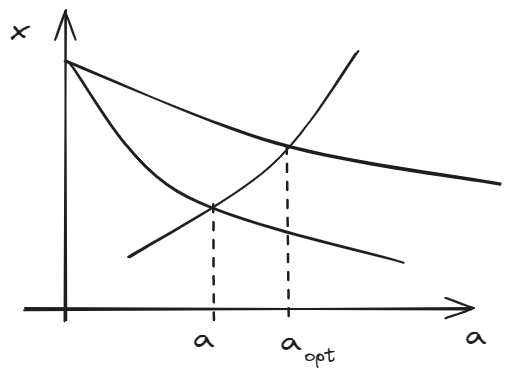
\includegraphics[width=0.5\textwidth]{assets/economics/shared.excalidraw.png}
    \caption{Принципал повышает эффективность труда}
    \label{ineficacy}
\end{figure}

Задача постановки определить правила заключается в определении условий на оплату труда, обеспечивающие
максимум коллективного удовлетворения(\textit{англ.} social plan):
\begin{equation}
    \max_{a_1, \dots, a_n} \sum^{i=1}^n \left[\omega_i(Q) - g_i(a_i) \right]
\end{equation}

Обозначим максимум функции производства, соответствующий максимизации, как $\hat{Q}$ и $\mathbf{a}_i$.
Получим связь переменных из условия равенства нулю производной в точке максимума: 
\begin{equation}
    \sum_{i=1}^n\frac{\partial w_i(Q)}{\partial Q } \cdot \frac{\partial Q}{\partial a_i} = g_i'(a_i) 
\end{equation}



В отсутствие механизма принципала агенты максимизируют свое собственное счастье:
\begin{equation}
    \max_{a_i} \omega_i(Q) - g_i(a_i)
\end{equation}
Тогда вклад агента $a_i$ будет задан как:

\begin{equation}
    \frac{\partial w_i(Q)}{\partial Q } \cdot \frac{\partial Q}{\partial a_i} - g_i'(a_i) =0 
\end{equation}


Для коллектива

Принципал разрешает проблему задавая правило оплаты труда согласно достижению $Q$ общего социального максимума  

Тогда вклад агента $a_i$ будет задан как:






$$
    \max_{a_1}
$$




